\documentclass[conference]{IEEEtran}
\IEEEoverridecommandlockouts
% The preceding line is only needed to identify funding in the first footnote. If that is unneeded, please comment it out.
\usepackage{cite}
\usepackage{amsmath,amssymb,amsfonts}
\usepackage{algorithmic}
\usepackage{graphicx}
\usepackage{textcomp}
\usepackage{fancyhdr}
\usepackage{xcolor}
\pagestyle{fancy}
\def\BibTeX{{\rm B\kern-.05em{\sc i\kern-.025em b}\kern-.08em
    T\kern-.1667em\lower.7ex\hbox{E}\kern-.125emX}}



\begin{document}
\leftmark{github hash: 364e69b8665f1d21354fa25a20ebb4d10bea507f}


\title{Desperately Seeking Sutton\\
% {\footnotesize \textsuperscript{*}Note: Sub-titles are not captured in Xplore and
% should not be used}
% \thanks{Identify applicable funding agency here. If none, delete this.}
}

\author{\IEEEauthorblockN{Tiantian Guo}
% \IEEEauthorblockA{\textit{dept. name of organization (of Aff.)} \\
% \textit{name of organization (of Aff.)}\\
% City, Country \\
\textit{tguo60@gatech.edu}
}

\maketitle

\begin{abstract}
This report will reproduce Richard Sutton's 1988 paper\cite{b1} three figures in order to augments the understanding of the paper and extend existing literature.
\end{abstract}

\begin{IEEEkeywords}
reinforcement learning, temporal differences, incremental learning
\end{IEEEkeywords}

\section{Introduction}
The paper "Learning to Predict by the Methods of Temporal Differences" \cite{b1} proved that for most real-world prediction problems, temporal-difference methods require less memory and less peak computation than conventional supervised learning methods and they even produce more accurate predictions. This report implements \cite{b1} experiments to better understanding TD-learning.

\section{Problem Statement}
A bounded random walk in a state sequence generated by taking random steps to the right or to the left until a boundary is reached. Fig.~\ref{fig1} shows a system that generates such state sequences. There are seven states ($A$, $B$, $C$, $D$, $E$, $F$, $G$) in random walks. Every walk begins in the center state $D$. At each step the walk moves to the neighboring state, either to the right or to the left with equal probability. If either edge state ($A$ or $G$) is entered, the walk terminates. 

\begin{figure}[htbp]
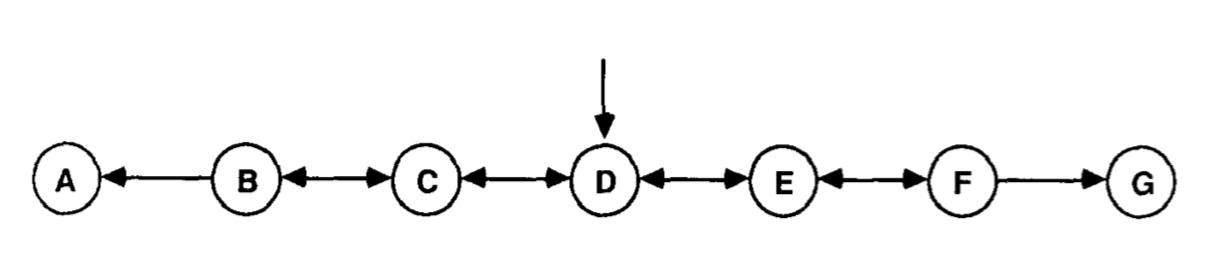
\includegraphics[width=\linewidth]{randomwalk.png}
\caption{A generator of bounded random walk.}
\label{fig1}
\end{figure}

A walk's outcome was defined to be $z = 0$ for a walk ending on the left at $A$ and $z = 1$ for a walk ending on the right at $G$. The random walk learning methods estimated the expected value of outcome $z$, the expected value is equal to the probability of a right-side termination. Ideal predictions for non-terminal states are $\{\frac{1}{6}, \frac{1}{3}, \frac{1}{2}, \frac{2}{3}, \frac{5}{6}\}$. The random walk outcome is the expected value of $z$, in this problem, its expected value is equal to the probability of a right-side termination. 

For each nonterminal state $i$, the observation vector $\textbf{x}_i$, which will set the walk position as 1, others as 0, e.g. $\textbf{x}_D$ = $(0,0,1,0,0)^T$. The prediction can be calculated as $P_t = \omega^Tx_t$ and $P_{m+1} = z$. When termination is state $A$, $z = 0$ while $z = 1$ when termination is state $G$.

TD($\lambda$) is used to estimate probability of right-side termination. In TD($\lambda$), learning procedure is summarized as follows:

\begin{equation}\label{eqn:1}
    \omega \leftarrow \omega + \sum_{m}^{t=1}\Delta \omega_t
  \end{equation}

\begin{equation}\label{eqn:2}
    \Delta \omega_t = \alpha (P_{t+1}-P_t)\sum_{t}^{k=1}\lambda ^{t-k}\bigtriangledown _\omega P_k
\end{equation}

\begin{equation}\label{eqn:3}
    P_t = \omega^Tx_t
\end{equation}


(\ref{eqn:1}) is the updated process of the weight $\omega$. (\ref{eqn:2}) is the calculation of the change of $\omega$, $\alpha$ is a positive parameter affecting the rate of learning and $\lambda$ is an exponential weighting with recency, in which alterations to the predictions of observation vectors occurring $k$ steps in the past are weighted according to $\lambda^k$ for $0 \leq \lambda \leq 1$. At $\lambda = 1$, TD(1), the algorithm simplifies to supervised learning. In (\ref{eqn:3}), $P_t$ was simply the value  of the $i^{th}$ component of $\omega$. To treat this problem simpler, $\bigtriangledown_\omega P_k = x_t$. Predictions or weight vectors are learnt by accumulating changes in weights per each time step. 

This project is to evaluate the relationship between weights $\omega$ estimation error, $\alpha$ and $\lambda$ under different experiment settings in \ref{sec:1}, \ref{sec:2} and \ref{sec:3}.

\section{Experiment 1 - Repeated Presentation}\label{sec:1}

\subsection{Settings}
This experiment computes average error on the random-walk problem under repeated training. In order to obtain statistically reliable results, 100 training sets, each consisting of 10 random walk sequences, were constructed for all learning procedures. For all procedures, weight increments were computed according to TD($\lambda$), as in (\ref{eqn:1}). Seven values were used for $\lambda$. $\lambda = 1$ is refering to Widrow-Hoff supervised-learning, $\lambda = 0$ is TD(0), and $\lambda = 0.1, 0.2, 0.3, 0.4, 0.5, 0.6, 0.7, 0.8, 0.9, 1.0$. $\omega$ weight vector is initialized to [0.5,0.5,0.5,0.5,0.5].

In this experiment, the weight vector was not updated after each sequence as indicated by (\ref{eqn:1}). The $\Delta \omega$'s were accumulated over sequences and only used to update the weight vector after a training set. Each training set was presented repeatedly to each learning procedure until the $\Delta\omega$ converge. If total $\Delta\omega$ is greater than 0.001, same training set is used until weights converge. $\alpha$ values are chosen from 0.001 to 0.01 with 0.0005 interval. $\alpha$ produces smallest $\Delta\omega$ is finally used in plotting Fig.~\ref{fig2}.

\subsection{Result}

\begin{figure}[htbp]
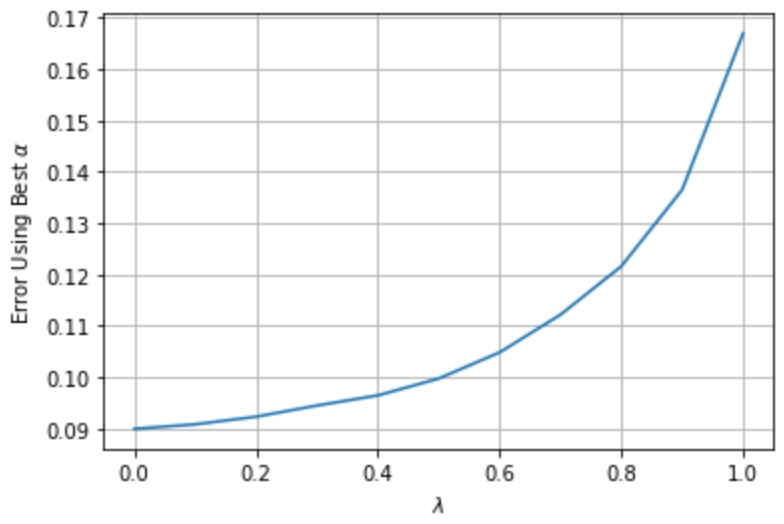
\includegraphics[width=\linewidth]{output1.png}
\caption{Average error on the random-walk problem under repeated presentations. All data are from TD($\lambda$) with different values of $\lambda$}
\label{fig2}
\end{figure}

The dependent measure used is the RMS error between the ideal predictions and those found by the learning procedure after being repeatedly presented with the training set until convergence of the weight vector. Results are generated as Fig.~\ref{fig2} (with $\alpha$ generates best RMSE among 100 training set each with 10 sequences). The $\alpha$ produces best error is listed in Table.I.

As shown, result is similar to Figure 3 in Sutton paper, in which RSME error exponentially increases as $\lambda$ reaches 1. TD(0) is converging to optimal predictions, outperforming Widrow-Hoff or TD(1).

However, the RMSE value in this experiment is slightly lower than Sutton's. The difference is mainly due to convergence limit settings or other settings that not explicitly explained.

\begin{table}
\begin{center}
 \begin{tabular}{||c c ||} 
 \hline
 $\lambda$ & Best $\alpha$ \\ [0.5ex] 
 \hline\hline
 0.0 - 0.3  & 0.002  \\
 \hline
 0.4 - 0.7  & 0.0015  \\
 \hline
 0.8 - 1.0 & 0.001  \\ [1ex]
 \hline
\end{tabular}
\end{center}
 \caption{Best $\alpha$ in repeated training}
\end{table}

\subsection{Pitfalls}

Sutton's paper does not explicitly define convergence condition and learning rate. Also the limit in number of steps or training sequences also remain unknown.

\section{Experiment 2 - Learning Rate Analysis}\label{sec:2}

\subsection{Settings}
This experiment setting is similar as the experiment 1, but concerns of learning rate when the training set is presented just once rather than repeatedly until convergence. Weights $\omega$ are updated after each sequence but will not training till convergence. $\alpha$ and $\lambda$ are both variables in this experiment.

\subsection{Result}

As shown in Fig.~\ref{fig3}, RMSE curves are shifted left from Sutton's work by about 0.1$\alpha$, but the shape and trend are similar. This difference maybe because of various length of training sequences. Larger training sequences maybe can produce more similar plot as Sutton's result.

\begin{figure}[htbp]
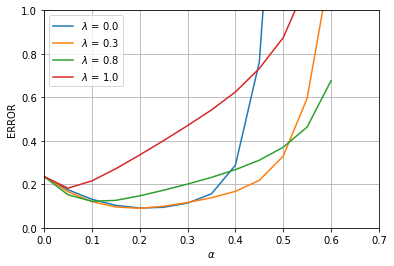
\includegraphics[width=\linewidth]{output2.png}
\caption{Average error on random walk problem after experiencing 10 sequences.}
\label{fig3}
\end{figure}

\subsection{Pitfalls}

This experiment does not place a steps limitations in random walk sequences. 

\section{Experiment 3 - Best $\alpha$ Analysis}\label{sec:3}

\subsection{Settings}
Same settings as Section~\ref{sec:2}, this experiments examine minimal RSME for each $\lambda$ using best $\alpha$ determined. Each data point represents teh average over 100 training sets of the error in the estimates found by TD($\lambda$), for particular $\lambda$  and $\alpha$ values, after a single presentation of a training set. The $\lambda$ value is given by horizontal coordinate. The $\alpha$ value was selected from those shown in Fig.\ref{fig3} to yield the lowest error for that $\lambda$ value.

\subsection{Result}

The best $\alpha$ can be calculated as in Table.II. This experiment produces similar result, as seen in Fig.\ref{fig4} to Sutton's paper but a little difference in the optimal $\lambda$. This result demonstrate that the single training has slower learning as best $\lambda$ is not the same as in Fig.\ref{fig2}.

\begin{figure}[htbp]
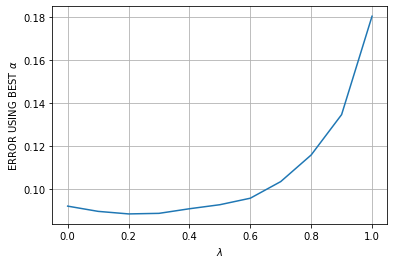
\includegraphics[width=\linewidth]{output3.png}
\caption{Average error at best $\alpha$ value on random-walk problem.}
\label{fig4}
\end{figure}

\begin{table}
\begin{center}
 \begin{tabular}{||c c ||} 
 \hline
 $\lambda$ & Best $\alpha$ \\ [0.5ex] 
 \hline\hline
0.0 - 0.4  & 0.2  \\ 
 \hline
0.5 - 0.7  & 0.15  \\
 \hline
0.8 - 0.9 & 0.1  \\ [1ex]
 \hline
0.1 & 0.005  \\ [1ex]
 \hline
\end{tabular}
\end{center}
\caption{Best $\alpha$ in non-repeated training}\label{tab:2}
\end{table}

\subsection{Pitfalls}
Sutton does not explicity present initial values of weight vector. Also as previously, the experiment assumes linear prediction.

\section{Conclusion}

Three implementation results are very similar to Sutton's paper. However, the differences between Sutton's plots and this report's plot maybe due to initial value of weights $\omega$, weight updating procedure, training set repeatation will significantly affects performance.


\begin{thebibliography}{00}
\bibitem{b1} Sutton, R.S , ``Learning to predict by the methods of temporal differences,'' Machine Learning, 3, pages9–44(1988), 1988.
\end{thebibliography}
\vspace{12pt}

\end{document}
